\chapter{Lecture 5: New Revolutions in Particle Physics: Basic Concepts}

These notes follow Leonard Susskind's fifth lecture in \emph{Particle Physics 1: Basic Concepts}, in a format curated by LazyingArt LLC. The lecture begins from a live question about waves, and that is already instructive. Before we can talk usefully about fermions, many-body ground states, and antiparticles, we have to sort out a prior issue: when a wave carries a particle, which part of the wave motion is actually physical, and which part is only a feature of the way we have written the phase? From there the lecture pauses for a compact symmetry recap, then turns to the algebra of exclusion, the Fermi sphere, hole excitations, and finally the simplest one-dimensional version of Dirac's logic.

\section{Phase Velocity, Group Velocity, and What Is Actually Measured}

The opening question is about phase velocity and group velocity. Susskind's first move is not to answer abstractly but to start with the simplest wave he can write:
\begin{equation}
\psi(x,t)=e^{i(kx-\omega t)},
\end{equation}
or, if we prefer a real wave,
\begin{equation}
\psi(x,t)=\sin(kx-\omega t).
\end{equation}
A crest, or more generally any point of fixed phase, moves so that
\begin{equation}
kx-\omega t=\text{const.}
\end{equation}
Hence
\begin{equation}
x=\frac{\omega}{k}\,t,
\qquad
v_{\mathrm{phase}}=\frac{\omega}{k}=\frac{\lambda}{T}.
\end{equation}
So the phase velocity is simply the speed at which constant phase moves.

For a nonrelativistic Schr\"odinger wave we use, after correcting the spoken slip in the lecture,
\begin{equation}
\omega=\frac{k^2}{2m}.
\end{equation}
Therefore
\begin{equation}
v_{\mathrm{phase}}=\frac{\omega}{k}=\frac{k}{2m}.
\end{equation}
But the classical particle velocity for momentum \(p=k\) is \(p/m=k/m\). There is an extra factor of two. The lecture does not immediately resolve that mismatch; it lets it stand for a moment as a warning that the motion of phase is not yet the motion of the particle.

\subsection{Question \& Answer}

\paragraph{Question.} Why can changing \(\omega\) by a constant alter the phase velocity without changing the physics?

\paragraph{Answer.} This is where the lecture deliberately undercuts the naive interpretation of phase motion. Write the Schr\"odinger field schematically as
\begin{equation}
\psi(x,t)=\sum_k c_k\,e^{ikx}e^{-i\omega(k)t},
\end{equation}
with normalization factors suppressed, just as they are suppressed in the lecture. Now shift every frequency by the same constant:
\begin{equation}
\omega(k)\longrightarrow \omega(k)+c.
\end{equation}
Every term in the sum acquires the same extra factor, so
\begin{equation}
\psi(x,t)\longrightarrow e^{-ict}\psi(x,t).
\end{equation}
But the physically interesting quantities are built from \(\psi\) and \(\psi^\ast\). In particular,
\begin{equation}
\psi(x,t)\psi^\ast(x,t)\longrightarrow
e^{-ict}e^{ict}\,\psi(x,t)\psi^\ast(x,t)
=
\psi(x,t)\psi^\ast(x,t).
\end{equation}
So the observables are unchanged. The shift merely adds a common time-dependent phase.

The phase velocity, however, becomes
\begin{equation}
v_{\mathrm{phase}}\longrightarrow \frac{\omega+c}{k}
=
v_{\mathrm{phase}}+\frac{c}{k}.
\end{equation}
Thus the phase velocity changes even though the measurable physics does not. This is the lecture's first real conclusion: for Schr\"odinger waves, phase velocity is not a reliable physical propagation speed. It is partly a matter of convention.

\section{Wave Packets and the Motion of Constructive Interference}

Once the phase velocity has been made suspect, the lecture asks what quantity really tracks physical motion. The answer is the group velocity, but Susskind does not announce it as a slogan. He derives it from the way a localized wave packet is built.

A packet is a superposition of plane waves. Its localization comes from interference: the waves add in one region and cancel elsewhere. To see the essential mechanism, it is enough to take two neighboring waves,
\begin{equation}
\psi(x,t)=\sin(kx-\omega t)+\sin(k'x-\omega' t),
\end{equation}
where \(k'\) is close to \(k\), and \(\omega'=\omega(k')\). The strongest constructive interference occurs where the two phases agree:
\begin{equation}
kx-\omega t=k'x-\omega' t.
\end{equation}
Rearranging,
\begin{equation}
(k-k')x=(\omega-\omega')t.
\end{equation}
So the moving locus of constructive interference obeys
\begin{equation}
x=\frac{\omega-\omega'}{k-k'}\,t.
\end{equation}
When \(k'\) approaches \(k\), this becomes
\begin{equation}
x=\frac{d\omega}{dk}\,t,
\qquad
v_{\mathrm{group}}=\frac{d\omega}{dk}.
\end{equation}
This is the group velocity: the velocity of the envelope, the lump, the place where the waves reinforce each other.

Now let us go back to the nonrelativistic dispersion relation, keeping the same additive constant that the lecture used to test the meaning of phase motion:
\begin{equation}
\omega=\frac{k^2}{2m}+c.
\end{equation}
Then
\begin{equation}
v_{\mathrm{group}}=\frac{d\omega}{dk}=\frac{k}{m}.
\end{equation}
The extra constant disappears, and the answer is exactly the classical particle velocity. This is the point Susskind wanted to get to: group velocity, unlike phase velocity, survives the additive-energy test and reproduces the expected particle motion.

\begin{figure}
\centering

\includegraphics[width=0.72\textwidth]{lecture_05_figure_03.png}
\caption{Board evidence for the opening wave discussion: the nonrelativistic dispersion \(\omega=k^2/(2m)+c\), the relativistic square-root relation, the ratio \(\omega/k\), and the derivative \(d\omega/dk\) written separately as the physically significant velocity.}
\end{figure}

\section{Relativistic Dispersion and the Superluminal Phase-Velocity Puzzle}

The lecture then broadens the discussion to a relativistic particle, partly because a student raises the familiar worry about waves whose phase seems to move faster than light. Here again the safest route is not rhetoric but calculation. With \(\hbar=c=1\),
\begin{equation}
E=\sqrt{p^2+m^2},
\qquad
\omega=\sqrt{k^2+m^2}.
\end{equation}
The phase velocity is
\begin{equation}
v_{\mathrm{phase}}=\frac{\omega}{k}
=
\sqrt{\frac{k^2+m^2}{k^2}},
\end{equation}
which is greater than \(1\) whenever \(m\neq 0\). That is the moment where one is meant to feel a small alarm: the phase seems to outrun light.

But the group velocity is
\begin{equation}
v_{\mathrm{group}}=\frac{d\omega}{dk}
=
\frac{k}{\sqrt{k^2+m^2}}
=
\sqrt{\frac{k^2}{k^2+m^2}},
\end{equation}
which is always less than \(1\). In this particular example,
\begin{equation}
v_{\mathrm{phase}}v_{\mathrm{group}}=1.
\end{equation}
The lecture remarks that this inverse relation is not a general theorem. It is a special property of this dispersion relation.

What \emph{is} general is the role of dispersion. If \(\omega\) is proportional to \(k\), then every Fourier component moves with the same speed and the packet does not spread. If \(\omega\) is nonlinear in \(k\), different components move differently, and the packet changes shape in time. That is why the distinction between phase and group velocity is tied to the broader phenomenon of dispersion.

A massless particle in vacuum provides the clean limiting case. There \(\omega=|k|\), so on one branch \(\omega=k\), and then both the phase and group velocities are equal to \(1\). In that linear case there is no dispersion to distinguish them.

\section{Translation Symmetry, Phase Symmetry, and Conservation Laws}

Before moving on to fermions, the lecture pauses to re-anchor the discussion in the language of amplitudes. This is a quick review, but it matters: the lecture wants the transition from wave kinematics to particle physics to feel continuous.

Suppose a scattering amplitude has been reduced, after the field operators act, to a time-dependent factor of the form
\begin{equation}
\mathcal{A}(t)\propto
\exp\!\left[
i\left(
\sum \omega_{\mathrm{out}}-\sum \omega_{\mathrm{in}}
\right)t
\right].
\end{equation}
If the interaction can occur with equal amplitude at any time, we integrate over all time:
\begin{equation}
\int dt\,\mathcal{A}(t)\propto
\delta\!\left(
\sum \omega_{\mathrm{out}}-\sum \omega_{\mathrm{in}}
\right).
\end{equation}
This is the lecture's compact demonstration of energy conservation from time-translation invariance.

Momentum conservation is the same logic with space replacing time. For a simple decay \(k\to k_1'+k_2'\), the position dependence of the amplitude carries the factor
\begin{equation}
\mathcal{A}(x)\propto e^{i(k-k_1'-k_2')x}.
\end{equation}
If the process can happen with equal amplitude anywhere in space, we integrate over all \(x\):
\begin{equation}
\int dx\,\mathcal{A}(x)\propto \delta(k-k_1'-k_2').
\end{equation}
In the many-particle case this becomes
\begin{equation}
\int dx\,\mathcal{A}(x)\propto
\delta\!\left(
\sum k_{\mathrm{out}}-\sum k_{\mathrm{in}}
\right).
\end{equation}
So momentum conservation comes from space-translation invariance in exactly the same way that energy conservation comes from time-translation invariance.

There is then a third symmetry:
\begin{equation}
\psi\longrightarrow e^{i\lambda}\psi.
\end{equation}
A global phase rotation of this sort does not change amplitudes as long as the same number of \(\psi\)'s and \(\psi^\dagger\)'s appear. For a charge-carrying field, the lecture wants us to read that invariance as charge conservation. In particular, if \(\psi\) is an electron field, invariance under a global phase change goes hand in hand with the statement that the net electric charge is conserved.

The board evidence in this part of the lecture is partial and not fully legible, so the formulas above are written in cleaned form from the transcript.

\begin{figure}
\centering

\includegraphics[width=0.58\textwidth]{lecture_05_figure_02.png}
\caption{A partial board trace from the symmetry recap, showing the time-integral structure and phase factors behind the energy-conservation argument. The final equations are best typeset directly from the transcript.}
\end{figure}

\section{Fermions, Anticommutators, and the Meaning of Exclusion}

Now the lecture changes gear. Bosons can pile into a single state; more than that, they tend to do so. Fermions are different. They do not merely fail to bunch. They are forbidden from occupying the same state. This is the Pauli principle, and the operator algebra is the bookkeeping that expresses it.

Susskind writes the fermion field in the same style as the boson field:
\begin{equation}
\psi(x)=\sum_k c_k\,e^{ikx},
\qquad
\psi^\dagger(x)=\sum_k c_k^\dagger\,e^{-ikx}.
\end{equation}
The formal expansion is familiar. The difference lies in what the creation and annihilation operators are allowed to do.

To isolate the algebra, the lecture strips things down to a single one-particle state. There are only two possibilities: the state is empty or occupied. We denote them by \(|0\rangle\) and \(|1\rangle\). Then
\begin{align}
c^\dagger|0\rangle &= |1\rangle,
&
c^\dagger|1\rangle &= 0,
\\
c|0\rangle &= 0,
&
c|1\rangle &= |0\rangle.
\end{align}
Here the symbol \(0\) on the right is the zero vector, not the vacuum state \(|0\rangle\). The lecture insists on that distinction because otherwise the meaning of the algebra is obscured.

Now let us act with the combination \(c^\dagger c+cc^\dagger\). On \(|0\rangle\), the first term vanishes and the second returns \(|0\rangle\). On \(|1\rangle\), the second vanishes and the first returns \(|1\rangle\). Thus
\begin{equation}
\{c,c^\dagger\}=cc^\dagger+c^\dagger c=1.
\end{equation}
Likewise, trying to create twice in the same state, or annihilate twice from the same state, always gives zero:
\begin{equation}
\{c,c\}=0,
\qquad
\{c^\dagger,c^\dagger\}=0.
\end{equation}
For momentum-labelled states, the lecture generalizes this immediately to
\begin{equation}
\{c_k,c_{k'}^\dagger\}=\delta_{kk'},
\qquad
\{c_k,c_{k'}\}=0,
\qquad
\{c_k^\dagger,c_{k'}^\dagger\}=0.
\end{equation}
This is the fermionic analog of the bosonic commutator algebra, with commutators replaced by anticommutators.

The lecture then asks the right next question. If the algebra forbids two identical fermions from carrying the same momentum, does it also forbid them from being created at the same position? At \(x=0\) we have, schematically,
\begin{align}
\psi^\dagger(0)\psi^\dagger(0)|0\rangle
&=
\sum_{k,k'} c_k^\dagger c_{k'}^\dagger |0\rangle
\\
&=
\frac12\sum_{k,k'}
\left(
c_k^\dagger c_{k'}^\dagger
+
c_{k'}^\dagger c_k^\dagger
\right)|0\rangle
\\
&=
\frac12\sum_{k,k'}
\{c_k^\dagger,c_{k'}^\dagger\}|0\rangle
=0.
\end{align}
So the exclusion principle is not merely a statement about momentum labels. It excludes identical fermions from the same one-particle state altogether.

\begin{figure}
\centering

\includegraphics[width=0.74\textwidth]{lecture_05_figure_04.png}

\vspace{0.7em}

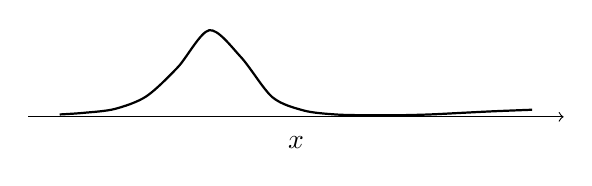
\begin{tikzpicture}[scale=1.0]
\draw[->] (-3.4,0) -- (3.4,0);
\draw[thick, smooth] plot coordinates {
(-3.0,0.03) (-2.7,0.05) (-2.3,0.10) (-1.9,0.26)
(-1.5,0.63) (-1.1,1.10) (-0.7,0.76) (-0.3,0.25)
(0.1,0.08) (0.5,0.03) (0.9,0.02) (1.3,0.02)
(1.7,0.03) (2.1,0.05) (2.5,0.07) (3.0,0.09)
};
\node at (0,-0.33) {$x$};
\end{tikzpicture}

\caption{Board evidence for the bridge from operator algebra to actual one-particle states: a localized wavefunction sketch at left, with creation-operator expressions at right. The curve is redrawn for clarity, but the screenshot is kept because the lecture's point depends on the juxtaposition of shape and operator bookkeeping.}
\end{figure}

\subsection{Question \& Answer}

\paragraph{Question.} What do we really mean by the same quantum state?

\paragraph{Answer.} This is the conceptual tightening that the lecture refuses to skip. A state is not, in general, specified by momentum alone. It may also involve spin; in an atom it involves an orbital wavefunction; in a beam it may be a localized packet rather than a plane wave. The correct statement is not ``same momentum'' but ``same quantum state.''

That is why the lecture turns to bound states and separated locations. Two electrons in different atoms may both be in what one informally calls a ground state, but the wavefunctions are different because one is centered here and the other there. They are not the same state.

The Nevada--Connecticut example makes the point even more sharply. Let \(|N\rangle\) be a state localized in Nevada and \(|C\rangle\) one localized in Connecticut. Then
\begin{equation}
|+\rangle=\frac{1}{\sqrt2}\bigl(|N\rangle+|C\rangle\bigr),
\qquad
|-\rangle=\frac{1}{\sqrt2}\bigl(|N\rangle-|C\rangle\bigr)
\end{equation}
are two distinct one-particle states. One electron may occupy \(|+\rangle\) and another may occupy \(|-\rangle\). What is forbidden is to put two electrons into the same state, say two electrons both in \(|+\rangle\).

This is also why the question ``Can two electrons have the same position but different momentum?'' is not well posed in the way ordinary language suggests. Position and momentum do not commute; they are not simultaneously sharp labels. A localized packet may have a fairly well-defined average momentum, but if we insist on making the momentum infinitely sharp, the localization is lost. The lecture is pressing us to use the word \emph{state} with care.

\section{Ground States: Boson Condensates, Fermi Spheres, and Holes}

Having clarified what exclusion really means, the lecture turns to the ground state of many-particle systems. The setting is a finite box. In one dimension, with periodic boundary conditions,
\begin{equation}
k=\frac{2\pi n}{L}.
\end{equation}
In three dimensions the allowed momentum vectors form a lattice in momentum space. Susskind draws only two dimensions on the board, but the intended picture is three-dimensional.

For bosons the ground state is immediate. Since
\begin{equation}
E=\frac{k^2}{2m},
\end{equation}
the lowest-energy one-particle state is \(k=0\). And because bosons may all occupy the same state, the many-body ground state puts every boson there. This is the boson condensate.

For fermions the first particle also goes into the lowest-energy state. But the next one cannot. Nor the next. To keep the total energy as low as possible, we must fill the available momentum states outward from the origin, one state at a time. In the large-volume limit the filled region is a sphere in momentum space, bounded by the Fermi surface. That filled region is the Fermi sphere; its interior is also called the Fermi sea.

\begin{figure}
\centering
\begin{tikzpicture}[scale=1.08]
\draw[->] (-3.8,0) -- (-0.8,0) node[right] {$k_x$};
\draw[->] (-2.3,-1.5) -- (-2.3,1.5) node[above] {$k_y$};
\fill (-2.3,0) circle (2.5pt);
\node at (-2.3,-1.95) {bosons};

\draw[->] (0.8,0) -- (3.8,0) node[right] {$k_x$};
\draw[->] (2.3,-1.5) -- (2.3,1.5) node[above] {$k_y$};
\draw[thick] (2.3,0) circle (1.0);
\fill (2.3,0) circle (1.8pt);
\fill (1.65,0) circle (1.6pt);
\fill (2.95,0) circle (1.6pt);
\fill (2.3,0.65) circle (1.6pt);
\fill (2.3,-0.65) circle (1.6pt);
\fill (1.95,0.35) circle (1.6pt);
\fill (2.65,0.35) circle (1.6pt);
\fill (1.95,-0.35) circle (1.6pt);
\fill (2.65,-0.35) circle (1.6pt);
\node at (2.3,-1.95) {fermions};
\end{tikzpicture}
\caption{Transcript-driven schematic of the contrasting ground states: bosons condensed at \(k=0\), and fermions filling outward in momentum space to a Fermi surface.}
\end{figure}

Now the lecture asks the next natural question: what is the cheapest excitation above the fermionic ground state? Not a deep rearrangement. Certainly not lifting an electron from the center of the Fermi sea all the way out, which would cost too much energy. The cheapest excitation is to take an electron from just below the Fermi surface and move it just above. That creates two low-energy excitations at once: a particle above the surface and a hole below it.

The transcript becomes a little ragged when the precise energy bookkeeping is discussed, but the stable point is clear if we measure energies relative to the Fermi surface. If \(\epsilon\) is the energy of the removed electron, \(\epsilon'\) the energy of the promoted one, and \(\epsilon_F\) the Fermi energy, then the excitation energy is naturally organized as
\begin{equation}
\Delta E
=
(\epsilon'-\epsilon_F)+(\epsilon_F-\epsilon),
\end{equation}
a sum of two positive quantities for a particle-hole excitation near the Fermi surface. One contribution belongs to the electron above the surface, the other to the hole below it.

The hole behaves as a positively charged excitation. It is literally an absence of negative charge, but at low energies it is more useful to treat it as a quasiparticle in its own right. When an electron drops into the hole, we may say either that the electron simply fell to a lower state or that the electron and the hole annihilated, with the released energy carried off by photons.

This point is sharpened by the lecture's discussion of photon absorption. A low-energy photon cannot excite an electron deep in the Fermi sea, because there is nowhere nearby for that electron to go; all the states below the surface are occupied, and the jump to an unoccupied state above the surface would cost too much energy. Low-energy photons therefore probe the neighborhood of the Fermi surface. In that sense the low-energy response is controlled by the surface of the Fermi sea, not by its volume.

\section{The Simplest One-Dimensional Dirac Logic}

At this point Susskind says explicitly what he has been aiming at: the hole story was already a story about antiparticles. The final section of the lecture translates that many-body idea into the simplest relativistic setting.

To keep the logic transparent, he works in one spatial dimension and takes a massless fermion-like field. The dispersion relation has two branches,
\begin{equation}
\omega=\pm k.
\end{equation}
Take first the branch \(\omega=k\). Now ask what differential equation has plane-wave solutions satisfying that relation. If
\begin{equation}
\psi(x,t)=e^{i(kx-\omega t)},
\end{equation}
then
\begin{equation}
\partial_t\psi=-i\omega\psi,
\qquad
\partial_x\psi=ik\psi.
\end{equation}
Therefore, when \(\omega=k\),
\begin{equation}
\partial_t\psi=-\partial_x\psi.
\end{equation}
This is the right-moving branch. The opposite sign gives
\begin{equation}
\partial_t\psi=+\partial_x\psi,
\end{equation}
which describes a left-moving branch.

\begin{figure}
\centering

\includegraphics[width=0.72\textwidth]{lecture_05_figure_05.png}

\vspace{0.7em}

\begin{tikzpicture}[scale=0.95]
\draw[->] (-2.4,0) -- (2.4,0) node[right] {$k$};
\draw[->] (0,-2.4) -- (0,2.4) node[above] {$\omega$};
\draw[thick] (-2.0,-2.0) -- (2.0,2.0) node[above right] {$\omega=k$};
\draw[thick,dashed] (-2.0,2.0) -- (2.0,-2.0) node[below right] {$\omega=-k$};
\end{tikzpicture}

\caption{The beginning of the one-dimensional Dirac-style derivation, paired with the two massless dispersion branches \(\omega=\pm k\). The screenshot preserves the live board start; the diagram makes the spectral structure explicit.}
\end{figure}

Now comes the dangerous feature. If \(\omega=k\), then negative \(k\) means negative \(\omega\), that is, negative energy. So the spectrum contains states of arbitrarily negative energy. If we started from an ordinary empty vacuum, positive-energy electrons could radiate and fall without bound to lower and lower energies. There would be no ground state.

\subsection{Question \& Answer}

\paragraph{Question.} How does filling the negative-energy sea turn the catastrophe into the vacuum and the hole into an antiparticle?

\paragraph{Answer.} The rescue uses the fact that the field is fermionic. A fermionic state can be occupied at most once. So instead of calling the state with no particles the vacuum, Dirac's move is to fill every negative-energy state and call that filled configuration the vacuum. Once every \(\omega<0\) state is occupied, there is nowhere lower for an electron to fall. The catastrophic cascade is blocked by exclusion.

From that vacuum we can create an excitation by lifting one negative-energy electron into a positive-energy state. Then two excitations appear. First, there is the positive-energy electron we have promoted. Second, there is the missing negative-energy electron left behind. That missing electron is the hole. Since it is an absence of negative charge, it carries positive charge. In this one-branch model it also carries positive momentum, because it is the deficit of a state of negative momentum.

This is the elementary content of the particle-antiparticle interpretation. Dirac's point is not that the hole is merely a bookkeeping fiction. It behaves as a genuine positively charged excitation of the vacuum.

At the same time, the lecture is careful about the limitations of the toy model. This is not yet the full Dirac equation. The particle here moves only in one direction; it moves at the speed of light; and it is massless. The model is meant only to isolate the central logical move. The later remark in the classroom about neutrinos should not be used to identify the toy model too literally.

The lecture also makes a sharp comparison with bosons. If we tried to use the same negative-energy picture for bosons, it would be a disaster. Bosons could pile into the negative-energy states without limit:
\begin{equation}
\text{fermions: at most one particle per state},
\qquad
\text{bosons: arbitrarily many particles per state}.
\end{equation}
So for bosons there would still be no ground state at all. In that sense the filled-sea rescue is not a generic quantum-field-theory trick; it is tied to fermionic exclusion.

\section{Summary}

The lecture unfolds along a very definite path. It begins with a question about wave motion and uses it to separate formal phase motion from physically meaningful propagation. The additive-constant test shows why phase velocity can be conventional, and the two-wave interference argument shows why the group velocity is the speed that tracks the packet and the particle.

From there the lecture briefly re-establishes the relation between symmetry and conservation laws before turning to fermions. Their anticommutator algebra is introduced not as an abstract axiom but as the bookkeeping of exclusion. That exclusion is then sharpened from ``same momentum'' to ``same quantum state,'' and the many-body consequences are drawn out in momentum space: bosons condense, fermions fill a Fermi sphere, and the cheapest fermionic excitations are particle-hole pairs near the Fermi surface.

The closing move is the conceptual payoff. The hole, first introduced as a low-energy excitation in a Fermi sea, becomes the prototype for the antiparticle in Dirac's relativistic logic. The lecture does not yet give the full Dirac equation, but it does give the essential idea: for fermions, a filled negative-energy sea can be reinterpreted as the vacuum, and a hole in that sea can appear as a positively charged particle.